\chapter{Requirements Specification and Analysis}

\section*{Introduction}

  In this chapter, we will present the analysis and specification of Requirements. We start by presenting the specification of the requirements, illustrating them using global use case diagram. Then we will present our project architecture and our working environment, and finally the product backlog and release planning, and we will close our chapter with a conclusion.

\section{Requirements Specification}

In this section, we will define the actors of our application and the functional and non-functional Requirements that our application aims to fulfill.

\subsection{Identifying Actors}

We define actors as a shorthand for the roles played by entities outside the system that interact directly with them \cite{CockburnUML2002}. In our system, we identify four types of actors:

\begin{itemize}
    \item \textbf{\textcolor{primary}{Super Admin}}: Responsible for the global configuration of the platform, they have extended privileges to manage administrators, oversee security, and ensure compliance. They can also configure advanced features and control all system resources.
    
    \item \textbf{\textcolor{primary}{Admin}}: In charge of the day-to-day management of the platform, they can add, modify, or delete listings, supervise agency and user profiles, and ensure smooth operations. They are also responsible for monitoring and assisting other actors.
    
    \item \textbf{\textcolor{primary}{Real Estate Agent}}: Dedicated to creating and updating real estate listings, they manage property information, handle investor requests, and finalize transactions related to sales or rentals. They can also coordinate property visits and propose tailored offers.
    
    \item \textbf{\textcolor{primary}{Investor}}: A user who wishes to browse and finance real estate projects. They have access to all available offers, can make investments in a few simple steps, and monitor the evolution of their portfolio. They also benefit from personalized insights to optimize their investments.
\end{itemize} 

\subsection{Functional Requirements}

After several meetings with our client, the various functional requirements of our application are illustrated as follows:

\subsubsection{For the Super Admin (Korpor)}
\begin{itemize}
    \item \textbf{Authenticate}: The super admin enters their credentials to access the advanced management console.
    \item \textbf{Log Out}: After viewing or updating global settings, they can securely log out.
    \item \textbf{Manage Admin Accounts}: Create, enable/disable, or modify admin profiles associated with different real estate companies.
    \item \textbf{Monitor Security \& Compliance}: Oversee transactions, data integrity, and regulatory adherence using specialized reporting and audit tools.
    \item \textbf{View Global Reports}: Generate and analyze consolidated metrics (financials, user activity, transactions) for overall performance insights.
    \item \textbf{Moderate Content}: Review and remove any inappropriate or erroneous property listings or user-generated data.
\end{itemize} 

\subsubsection{For the Admin (Real Estate Company)}
\begin{itemize}
    \item \textbf{Authenticate}: The admin logs in with valid credentials to manage daily operations.
    \item \textbf{Log Out}: They can end their session to maintain account security.
    \item \textbf{Manage Real Estate Listings}: Add, update, or delete property listings visible to investors.
    \item \textbf{Oversee Real Estate Agents}: Create and manage agent accounts, assign properties, and monitor performance and commissions.
    \item \textbf{Track Transactions \& Commissions}: Review incoming payments, calculate commissions owed to agents, and track the history of completed deals.
    \item \textbf{Address Investor Inquiries}: Respond to questions or concerns from investors, ensuring a smooth user experience.
    \item \textbf{Access Agency Dashboard}: View comprehensive statistics on properties, sales, rentals, and market trends.
\end{itemize}

\subsubsection{For the Real Estate Agent}
\begin{itemize}
    \item \textbf{Authenticate}: The agent logs in to manage assigned properties and interact with potential investors.
    \item \textbf{Log Out}: Securely exit the account after completing tasks.
    \item \textbf{Manage Assigned Properties}: Create new listings, update property details, set prices, and upload images.
    \item \textbf{Handle Investment Requests}: Review purchase or rental offers, negotiate terms, and initiate contract finalization.
    \item \textbf{Contribute to AI Estimates}: Provide or refine data to improve AI-driven pricing and market analysis.
    \item \textbf{Maintain Client Relationships}: Communicate with investors, schedule property visits, and follow up on inquiries.
    \item \textbf{View Commissions}: Track earnings based on successful sales or rentals.
\end{itemize}
\subsubsection{For the Investor (Mobile App User)}
\begin{itemize}
    \item \textbf{Create an account \& authenticate}: Register to gain access to the platform's core features.
    \item \textbf{Log Out}: End the session to protect personal and financial data.
    \item \textbf{Browse Listings \& Invest}: Explore available properties, filter according to preferences, and commit to an investment in a few steps.
    \item \textbf{Track Portfolio}: Monitor owned assets, property status, and receive real-time updates on performance.
    \item \textbf{Make Payments}: Use integrated payment methods (credit cards, digital wallets, etc.) to complete transactions.
    \item \textbf{Access AI Recommendations}: View data-driven insights and return-on-investment estimates generated by the system.
    \item \textbf{Manage Withdrawals \& Earnings}: Withdraw profits, monitor rental income, or exit investments under the right conditions.
\end{itemize} 

\subsection{Non-functional Requirements}

To ensure reliable decision-making and prevent anomalies, the solution must meet these non-functional requirements:
\begin{itemize}
    \item \textbf{Maintainability}: The system should be simple to update and fix \cite{DevOpsFoundation2023, FowlerRefactoring2018}.
    \item \textbf{Evolution}: The platform must adapt to user needs, improving services while maintaining efficiency \cite{PoppendieckLean2012, KnibergLeanStartup2013}.
    \item \textbf{Security}: Strong authentication, access control, and data encryption are required. Blockchain integration ensures data integrity \cite{WangBlockchainRealEstate2023}.
    \item \textbf{Efficiency}: The application must remain effective and reliable in all situations \cite{KimDevOpsMethods2018, BassArchitecture2021}.
    \item \textbf{Performance}: The system should be responsive and stable, even under heavy load or varying network conditions.
\end{itemize}

% \section*{Requirements Analysis}

% In this section, we'll outline the various features that our app should offer, using a general use case diagram \cite{CockburnUML2002}.

\subsection*{General use case diagram}

Below, we present the various actors of the application and the actions they are authorized to perform \ref{fig:use-case-diagram}.
% \newpage
\begin{figure}[htbp]
    \centering
    % Replace with actual image file once available
    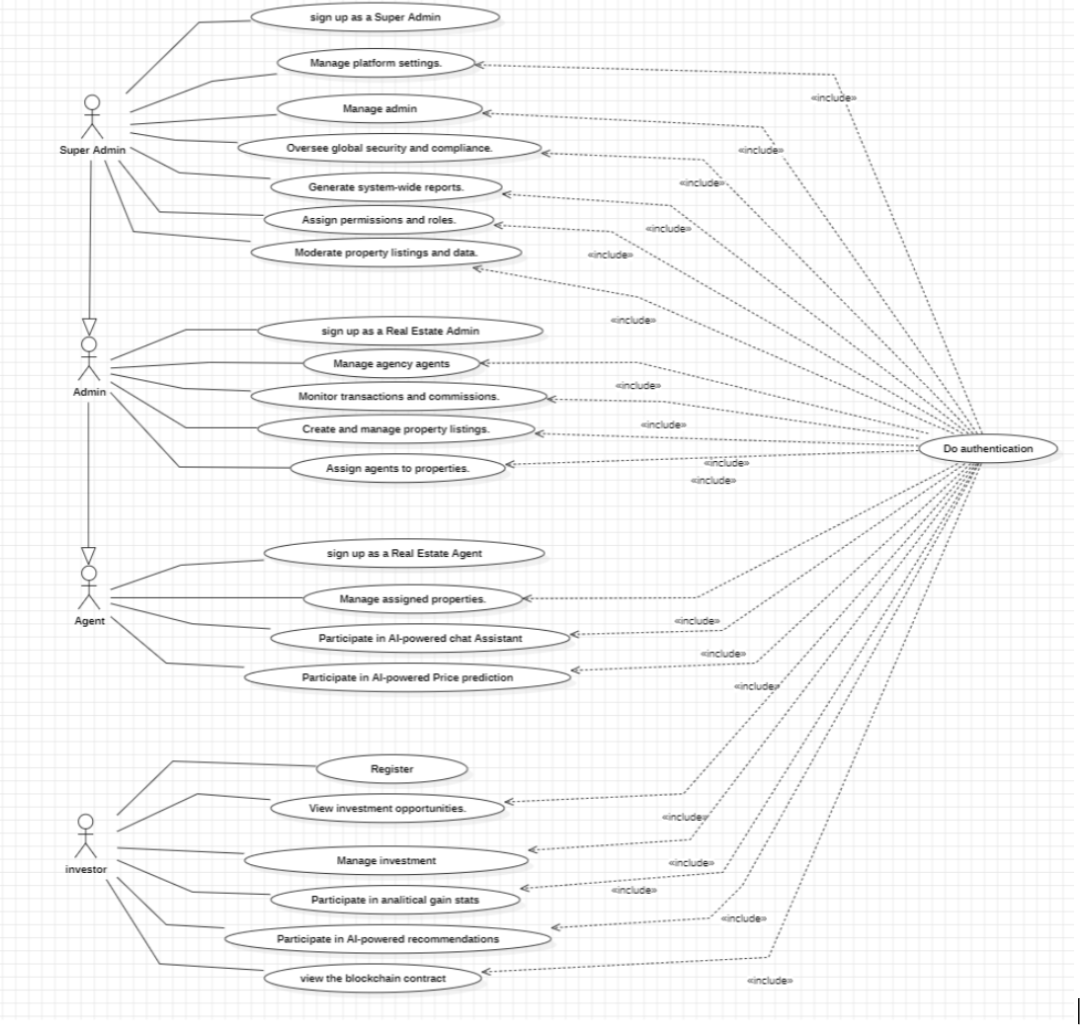
\includegraphics[width=1.03\textwidth]{images/diagram de case d utilisation general.png}
    % \vspace{0.5cm}
    \caption{General use case diagram}
    \label{fig:use-case-diagram}
\end{figure}
\section{Software architecture}

Before starting the design and development of any computerized system, it is essential to prepare the architecture.

\subsection{Physical architecture}

Korpor's physical architecture, depicted in Figure \ref{fig:physical-architecture}, is a distributed system. Users interact via \textbf{\textcolor{primary}{Mobile Devices}} (React Native app) and \textbf{\textcolor{primary}{Web Browsers}} (React components), communicating via HTTP/JSON with backend services primarily on \textbf{\textcolor{primary}{Google Cloud Platform}} (GCP). GCP handles core logic and data, featuring a \textbf{\textcolor{primary}{Cloud Run JS Server}} for the main backend, a \textbf{\textcolor{primary}{Cloud Run Flask Server}} for AI models (prediction, recommendation, chatbots), \textbf{\textcolor{primary}{ Cloud SQL}} for database storage, and a \textbf{\textcolor{primary}{Google Cloud VPS}} for data scraping models. Blockchain operations leverage \textbf{\textcolor{primary}{Infura}} for Solidity code and the \textbf{\textcolor{primary}{Sepolia Testnet}} for contracts, using RPC and HTTP/JSON. An administrative \textbf{\textcolor{primary}{Web Panel}} is hosted on a \textbf{\textcolor{primary}{Hosting.com server}}. 

\begin{figure}[htbp]
    \centering
    % Replace with actual image file once available
    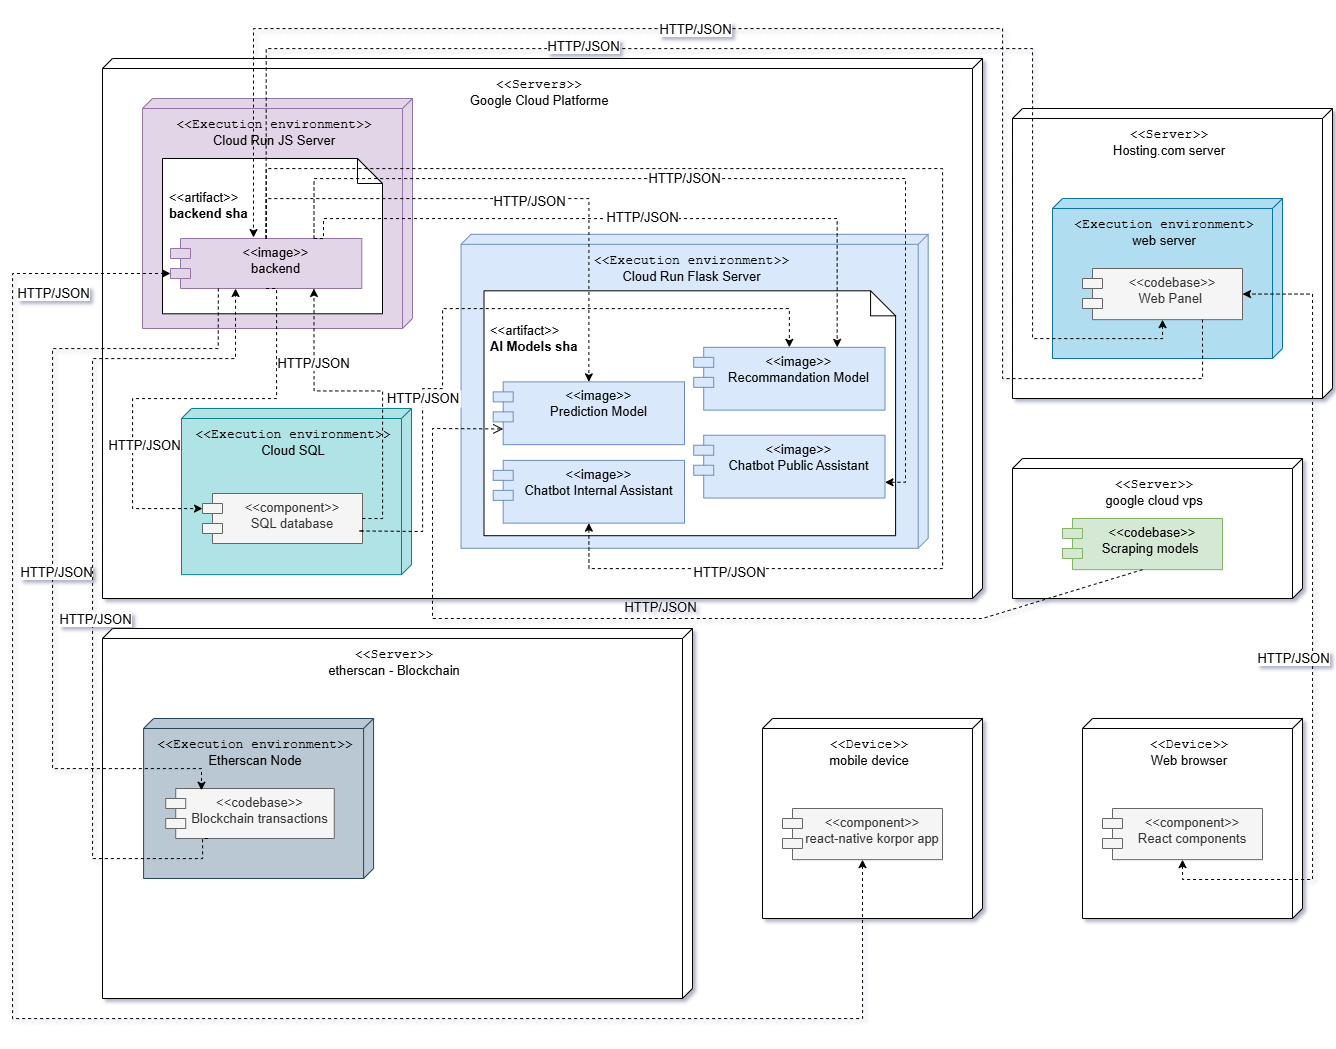
\includegraphics[width=1.03\textwidth]{images/deploiement_general_diag.png}
    % \vspace{0.5cm}  
    \caption{Deployment diagram}
    \label{fig:physical-architecture}
\end{figure}

\subsection{Logical architecture}

Korpor's logical architecture follows the MVC (Model-View-Controller) pattern \cite{SunardiMVC2019, GammaPatterns1994} for maintainability, with microservices principles applied for scalable system design \cite{NewmanMicroservices2021}.
\begin{itemize}
    \item \textbf{Model}: Manages application data and business logic, interacting with the backend database.
    \item \textbf{View}: The frontend (React, TypeScript, TanStack) presents data to users and handles interactions.
    \item \textbf{Controller}: The Express.js backend processes requests from the View, interacts with the Model and external services (Clerk, AI, Blockchain), and determines the response.
\end{itemize}
User requests flow from the View (frontend) to the Controller (backend), which interacts with the Model (data) and services before returning data to update the View. This structure ensures scalability and separation of concerns. The architecture is illustrated in Figure \ref{fig:logical-architecture}.
% \newpage

\begin{figure}[htbp]
    \centering
    % Replace with actual image file once available
    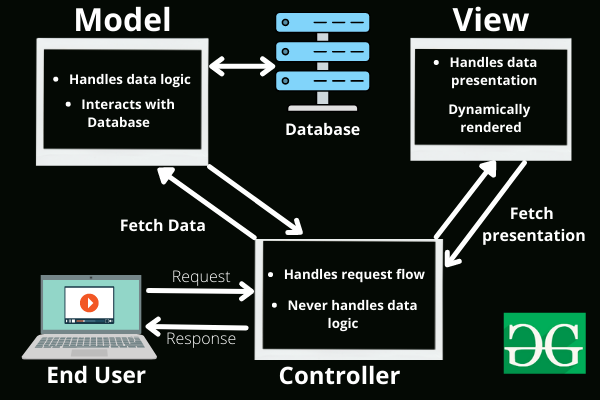
\includegraphics[width=0.8\textwidth]{images/logique.png}
    \caption{Logical architecture}
    \label{fig:logical-architecture}
\end{figure}

\section{Work Environment}

In this part, we will talk about our work environment, focusing on different aspects:
our material environment, the techniques we used in the realization of our project as well as the tools we used in our report, the product backlog and sprint planning, and finally, we will conclude this section \cite{BeckXP2004, MartinCleanArchitecture2017}.

\subsection{Physical environment}

The work was carried out by a laptop computer that is equipped with these detailed features presented in Table \ref{tab:physical-env} below:
\begin{table}[htbp]
    \centering
    \begin{tabular}{|l|l|}
        \hline
        \textbf{Computer Name} & MSI \\
        \hline
        \textbf{Processor} & i5 10th gen \\
        \hline
        \textbf{Hard disk} & 512 Go SSD \\
        \hline
        \textbf{RAM} & 24.0 Go \\
        \hline
        \textbf{Operating system} & Windows 11 Pro \\
        \hline
    \end{tabular}
    \caption{Physical environment}
    \label{tab:physical-env}
\end{table}


\subsection{Used technologies}

% Define a command for technology icons to make it easier to adjust if needed
\newcommand{\techicon}[1]{%
  \includegraphics[height=1em]{images/icons/#1.png}%
}

\subsubsection*{\protect\techicon{expo} Expo}

Expo is an open-source platform for making universal native apps for Android, iOS, and the web with JavaScript and React.

\subsubsection*{\protect\techicon{typescript} TypeScript}
                                                                
TypeScript (abbreviated as TS) is a free and open-source high-level programming language developed by Microsoft that adds static typing with optional type annotations to JavaScript. It is designed for the development of large applications and transpiles to JavaScript.

\subsubsection*{\protect\techicon{tanstack} Tanstack}
                                                                      
High-quality open-source software for web developers. Headless, type-safe, \& powerful utilities for Web Applications, Routing, State Management, Data Visualization, Datagrids/Tables, and more.

\subsubsection*{\protect\techicon{clerk}}
                                                                        
Clerk is a complete suite of embeddable UIs, flexible APIs, and admin dashboards to authenticate and manage your users.

\subsubsection*{\protect\techicon{maestro} Maestro}
                                                                        
Maestro is the simplest, most powerful, and most trusted end-to-end testing platform for mobile and web apps.

\subsubsection*{\protect\techicon{azure} Google cloud platform}

Google cloud platform, or just GCP, is the cloud computing platform developed by Google. It has management, access and development of applications and services to individuals, companies, and governments through its global infrastructure.

\subsubsection*{\protect\techicon{github} GitHub}

GitHub is a cloud-based service that helps developers store and manage their code, as well as track and control changes to their code.

\subsubsection*{\protect\techicon{express} Express.js}

Express.js is a minimal and flexible Node.js web application framework that provides a list of features for building web and mobile applications easily.

\subsubsection*{\protect\techicon{postman} Postman}

Postman is an API platform for building and using APIs. Postman simplifies each step of the API lifecycle and streamlines collaboration so you can create better APIs—faster.

\subsubsection*{\protect\techicon{vite} Vite}

Vite is a modern build tool that provides a fast and optimized development experience for React 17 applications. It leverages native ES modules and offers a highly efficient development server with hot module replacement (HMR).

\subsubsection*{\protect\techicon{react} React}

React, sometimes referred to as a frontend JavaScript framework, is a JavaScript library created by Facebook.

\subsubsection*{\protect\techicon{mysql} MySQL}

MySQL is an open-source relational database management system. It is based on structured query language (SQL), which is used to add, access and manage content in a database.

\subsubsection*{\protect\techicon{docker} Docker}

Docker is an open platform for developing, shipping, and running applications. Docker enables you to separate your applications from your infrastructure so you can deliver software quickly.

\subsubsection*{\protect\techicon{playwright} Playright}

Playwright is an open-source testing and automation framework that can automate web browser interactions. To put it simply, you can write code that can open a browser.

\subsubsection*{\protect\techicon{storybook} Storybook}

Storybook is a frontend workshop for building UI components and pages in isolation. It helps you develop and share hard-to-reach states and edge cases without needing to run your whole app.

\subsubsection*{\protect\techicon{staruml} StarUML}

StarUML is a sophisticated software modeler aimed to support agile and concise modeling. It provides eleven different types of diagrams and it accepts UML 2.x standards.

\subsubsection*{\protect\techicon{node} Node.js}

Node.js is an open-source, cross-platform JavaScript runtime environment that executes JavaScript code outside a web browser, allowing developers to use JavaScript for server-side scripting.


\subsection{Tools used for the report}

% Comment out problematic icon
\subsubsection*{\protect\techicon{overleaf} Overleaf}

Overleaf is a collaborative cloud-based LaTeX editor used to write, edit, and publish scientific papers.

% Comment out problematic icon
\subsubsection*{\protect\techicon{canva} Canva}

Canva is a global company that empowers people to design anything and publish anywhere. Learn about its mission, values, commitments, awards, product, and careers.


\subsection{Source code management with Git and GitHub}
GitHub was utilized for version control, employing a structured branching strategy for organized development. The `main` branch holds official release history, while `develop` serves as an integration branch for new features. Feature branches are created from `develop` for new tasks or bug fixes. Upon completion and testing, these are merged back into `develop` via pull requests, ensuring code review and quality control. Merging `develop` into `main` creates a new stable application version. This workflow is illustrated in Figure \ref{fig:git-workflow}.

\begin{figure}[ht!]
    \centering
    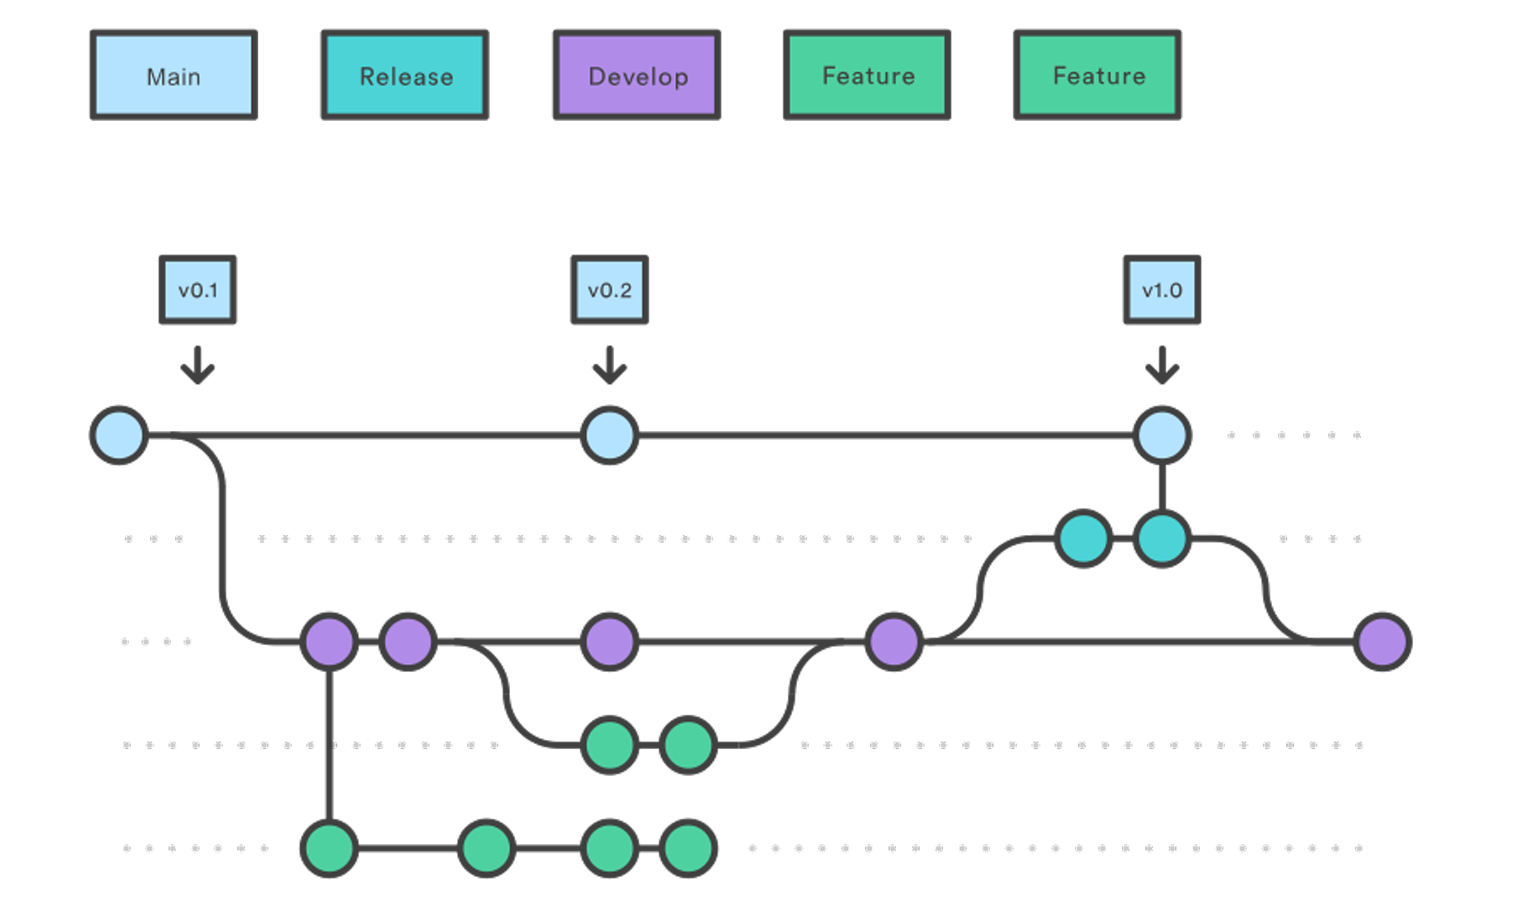
\includegraphics[width=0.9\textwidth]{images/gitWorkflow.png}
    \caption{Git Workflow}
    \label{fig:git-workflow}
\end{figure}


\section{Sprint Overview}

The project was organized into 8 focused sprints, each targeting specific functionality areas to deliver incremental value. The sprint planning ensured systematic development from core authentication to advanced AI and blockchain features Table \ref{tab:sprint-overview}.

\newpage
\begin{table}[ht!]
\centering
\caption{Korpor Project Sprint Overview\label{tab:sprint-overview}}
\begin{tabular}{|c|l|p{6cm}|c|}
\hline
\textbf{Sprint} & \textbf{Focus Area} & \textbf{Key Deliverables} & \textbf{Duration} \\
\hline
1 & Authentication \& User Management & Secure login, role-based access & 2 weeks \\
\hline
2 & Data Collection \& Scraping & Data collection, web scraping systems & 1 week \\
\hline
3 & Property Valuation Model & AI-powered property valuation and prediction & 2 weeks \\
\hline
4 & Real Estate Assistant & NLP chatbot for real estate legal assistance & 1 week \\
\hline
5 & Role-Based Backoffice & Agent management systems & 2 weeks \\
\hline
6 & Recommendation System & AI-powered investment recommendations & 1 week \\
\hline
7 & Blockchain Integration & Payment processing with blockchain & 2 weeks \\
\hline
8 & Property Management \& Portfolio & Listing management, investment tracking & 4 weeks \\
\hline
\end{tabular}
\end{table}

\section{Sprint planning}

To meet internship deadlines, we carefully planned key tasks, estimated timelines, and visualized the project with a GANTT chart. We also considered cost estimation and agile scaling for enterprise development (see Figure~\ref{fig:gantt-chart}).

\begin{figure}[htbp]
    \centering
    
    % First part: February - March (Sprints 1-5)
    \resizebox{\textwidth}{!}{%
    \begin{ganttchart}[
        % Chart style configuration
        hgrid,
        vgrid,
        time slot format=isodate,
        x unit=4mm,
        y unit title=8mm,
        y unit chart=6mm,
        title height=1,
        % Colors and styles
        title/.append style={fill=primary!10, font=\small\bfseries},
        bar/.append style={fill=primary!70},
        bar label font=\small\bfseries,
        milestone/.append style={fill=accent, rounded corners=2pt},
        group/.append style={fill=primary!30}
    ]{2025-02-01}{2025-03-31}
    
    % Time axis with month increments
    \gantttitlecalendar{year, month=shortname} \\
    
    % Sprint 1 (Feb 1-14, 2 weeks)
    \ganttbar{Sprint 1}{2025-02-01}{2025-02-14} \\
    
    % Sprint 2 (Feb 15-21, 1 week)
    \ganttbar{Sprint 2}{2025-02-15}{2025-02-21} \\
    
    % Sprint 3 (Feb 22-Mar 7, 2 weeks)
    \ganttbar{Sprint 3}{2025-02-22}{2025-03-07} \\
    
    % Sprint 4 (Mar 8-15, 1 week)
    \ganttbar{Sprint 4}{2025-03-08}{2025-03-15} \\
    
    % Sprint 5 (Mar 15-28, 2 weeks)
    \ganttbar{Sprint 5}{2025-03-15}{2025-03-28} \\
    
    \end{ganttchart}
    }
    
    \vspace{1cm} % Space between the two charts
    
    % Second part: April - May (Sprints 6-10)
    \resizebox{\textwidth}{!}{%
    \begin{ganttchart}[
        % Chart style configuration
        hgrid,
        vgrid,
        time slot format=isodate,
        x unit=4mm,
        y unit title=8mm,
        y unit chart=6mm,
        title height=1,
        % Colors and styles
        title/.append style={fill=primary!10, font=\small\bfseries},
        bar/.append style={fill=primary!70},
        bar label font=\small\bfseries,
        milestone/.append style={fill=accent, rounded corners=2pt},
        group/.append style={fill=primary!30}
    ]{2025-04-01}{2025-05-31}
    
    % Time axis with month increments
    \gantttitlecalendar{year, month=shortname} \\
    
    % Sprint 6 (Mar 29-Apr 4, 1 week) - Note: starts in March but extends to April
    \ganttbar{Sprint 6}{2025-04-01}{2025-04-04} \\
    
    % Sprint 7 (Apr 5-18, 2 weeks)
    \ganttbar{Sprint 7}{2025-04-05}{2025-04-18} \\
    
    % Sprint 8 (Apr 19-May 2, 2 weeks)
    \ganttbar{Sprint 8}{2025-04-19}{2025-05-16} \\
    
    
    
    
    \end{ganttchart}
    }
    
    \caption{GANTT chart with sprint planning (February - May 2025)}
    \label{fig:gantt-chart}
\end{figure}

\section*{Conclusion}

This chapter established the project's foundation, outlining our planning, architecture, and methodology for successful delivery.

\addtocontents{toc}{\protect\newpage}
